%%%%%%%% ICML 2025 EXAMPLE LATEX SUBMISSION FILE %%%%%%%%%%%%%%%%%

\documentclass{article}
\usepackage[T1]{fontenc}
% Recommended, but optional, packages for figures and better typesetting:
\usepackage{microtype}
\usepackage{graphicx}
\usepackage{subcaption}
\usepackage{booktabs} % for professional tables

% hyperref makes hyperlinks in the resulting PDF.
\usepackage{hyperref}

% Attempt to make hyperref and algorithmic work together better:
\newcommand{\theHalgorithm}{\arabic{algorithm}}

% If accepted, instead use the following line for the camera-ready submission:
\usepackage[accepted]{icml2025}

% Eliminar el texto de "Proceedings of ICML..." de la primera página
\makeatletter
\renewcommand{\ICML@appearing}{}
\makeatother

% For theorems and such
\usepackage{amsmath}
\usepackage{amssymb}
\usepackage{mathtools}
\usepackage{amsthm}

% if you use cleveref..
\usepackage[capitalize,noabbrev]{cleveref}

% Custom table spacing
\usepackage{tabla}

% For list customization
\usepackage{enumitem}
\setlist[itemize]{noitemsep, topsep=1pt, leftmargin=*}
\setlist[enumerate]{noitemsep, topsep=0pt, leftmargin=*}

% Pie de página personalizado en la última página
\usepackage{lastpage}
\makeatletter
\fancypagestyle{lastpagestyle}{%
  \fancyhf{}
  \fancyhead{}
  \chead{}
  \cfoot{\thepage\\[0.3cm]\small\hypertarget{author1}{}\textsuperscript{1}Jordi Blasco Lozano -- DNI: 74527208D -- jordiblloz@gmail.com}
  \renewcommand{\headrulewidth}{1pt}
}
\AtEndDocument{\thispagestyle{lastpagestyle}}
\makeatother

% The \icmltitle you define below is probably too long as a header.
\icmltitlerunning{Análisis Comparativo de Graph Neural Networks: GCN vs MLP}

\begin{document}

\twocolumn[
\icmltitle{Análisis Comparativo de Graph Neural Networks: GCN vs MLP \\ en Clasificación de Nodos}

\begin{icmlauthorlist}
\icmlauthor{Jordi Blasco Lozano\hyperlink{author1}{\textsuperscript{1}}}{}
\end{icmlauthorlist}

\icmlkeywords{GNN, GCN, Machine Learning, Deep Learning, Graphs}

\vskip 0.3in
]

\begin{abstract}
Este trabajo aborda la Práctica 1 sobre Graph Neural Networks (GNNs), enfocado en la clasificación de nodos. Se ha diseñado un experimento controlado mediante un dataset sintético basado en Stochastic Block Models (SBM), con características de nodo ruidosas para aislar y demostrar la importancia de la información estructural. Comparamos un Perceptrón Multicapa (MLP), que ignora la topología del grafo, frente a una Graph Convolutional Network (GCN), que utiliza el mecanismo de paso de mensajes (\textit{message passing}). Los resultados demuestran que, en presencia de características con baja relación señal-ruido, la capacidad de las GCN para agregar información del vecindario resulta crítica para el rendimiento, superando ampliamente al MLP. Adicionalmente, se valida el desempeño en datasets benchmark reales como Cora y Citeseer.
\end{abstract}

\section{Introducción y Motivación}
\label{introduction}

El aprendizaje profundo tradicional (Deep Learning) ha tenido un éxito inmenso en datos estructurados en rejillas euclidianas (i.e., imágenes con CNNs) o secuencias (i.e., texto con RNNs/Transformers). Sin embargo, muchos datos en el mundo real, como redes sociales, estructuras moleculares o redes de citas, se representan mejor como grafos, donde la conectividad es arbitraria y no euclidiana.

El objetivo principal de esta práctica es comprender empíricamente por qué y cuándo las \textbf{Graph Neural Networks (GNNs)} ofrecen una ventaja sobre las arquitecturas clásicas como los MLPs. Para ello, comparamos dos enfoques:
\begin{itemize}
    \item \textbf{MLP (Baseline):} Trata cada nodo como una instancia independiente ($iid$), utilizando solo sus características intrínsecas $\mathbf{x}_i$. Ignora completamente la matriz de adyacencia $\mathbf{A}$.
    \item \textbf{GCN (Propuesto):} Incorpora explícitamente la estructura del grafo, permitiendo que la representación de un nodo $\mathbf{h}_i$ dependa no solo de su $\mathbf{x}_i$, sino también de las características de sus vecinos $\mathcal{N}(i)$.
\end{itemize}

El concepto central que exploraremos es el de \textbf{homofilia} (nodos conectados tienden a ser similares) y cómo el mecanismo de \textit{message passing} permite "suavizar" el ruido de las características individuales aprovechando el contexto del vecindario.

\section{Metodología y Diseño Experimental}
\label{methodology}

\subsection{Generación del Dataset Sintético}
Para garantizar que la mejora en el rendimiento provenga del uso de la estructura y no de la calidad de las características, he diseñado un \textbf{Dataset Sintético Custom} con propiedades específicas:

\textbf{Estructura del Grafo (Topología):}
Utilicé un \textbf{Stochastic Block Model (SBM)} para generar un grafo de 2000 nodos divididos en 4 comunidades (clases).
\begin{itemize}
    \item $N=2000$ nodos, $C=4$ clases.
    \item Probabilidad intra-clase $p_{in}=0.02$: Alta probabilidad de conexión entre nodos de la misma clase.
    \item Probabilidad inter-clase $p_{out}=0.001$: Baja probabilidad de conexión entre clases distintas.
\end{itemize}
Esto crea una estructura de comunidades fuerte y clara, donde la vecindad es altamente informativa de la etiqueta de clase.

\begin{figure}[ht]
    \centering
    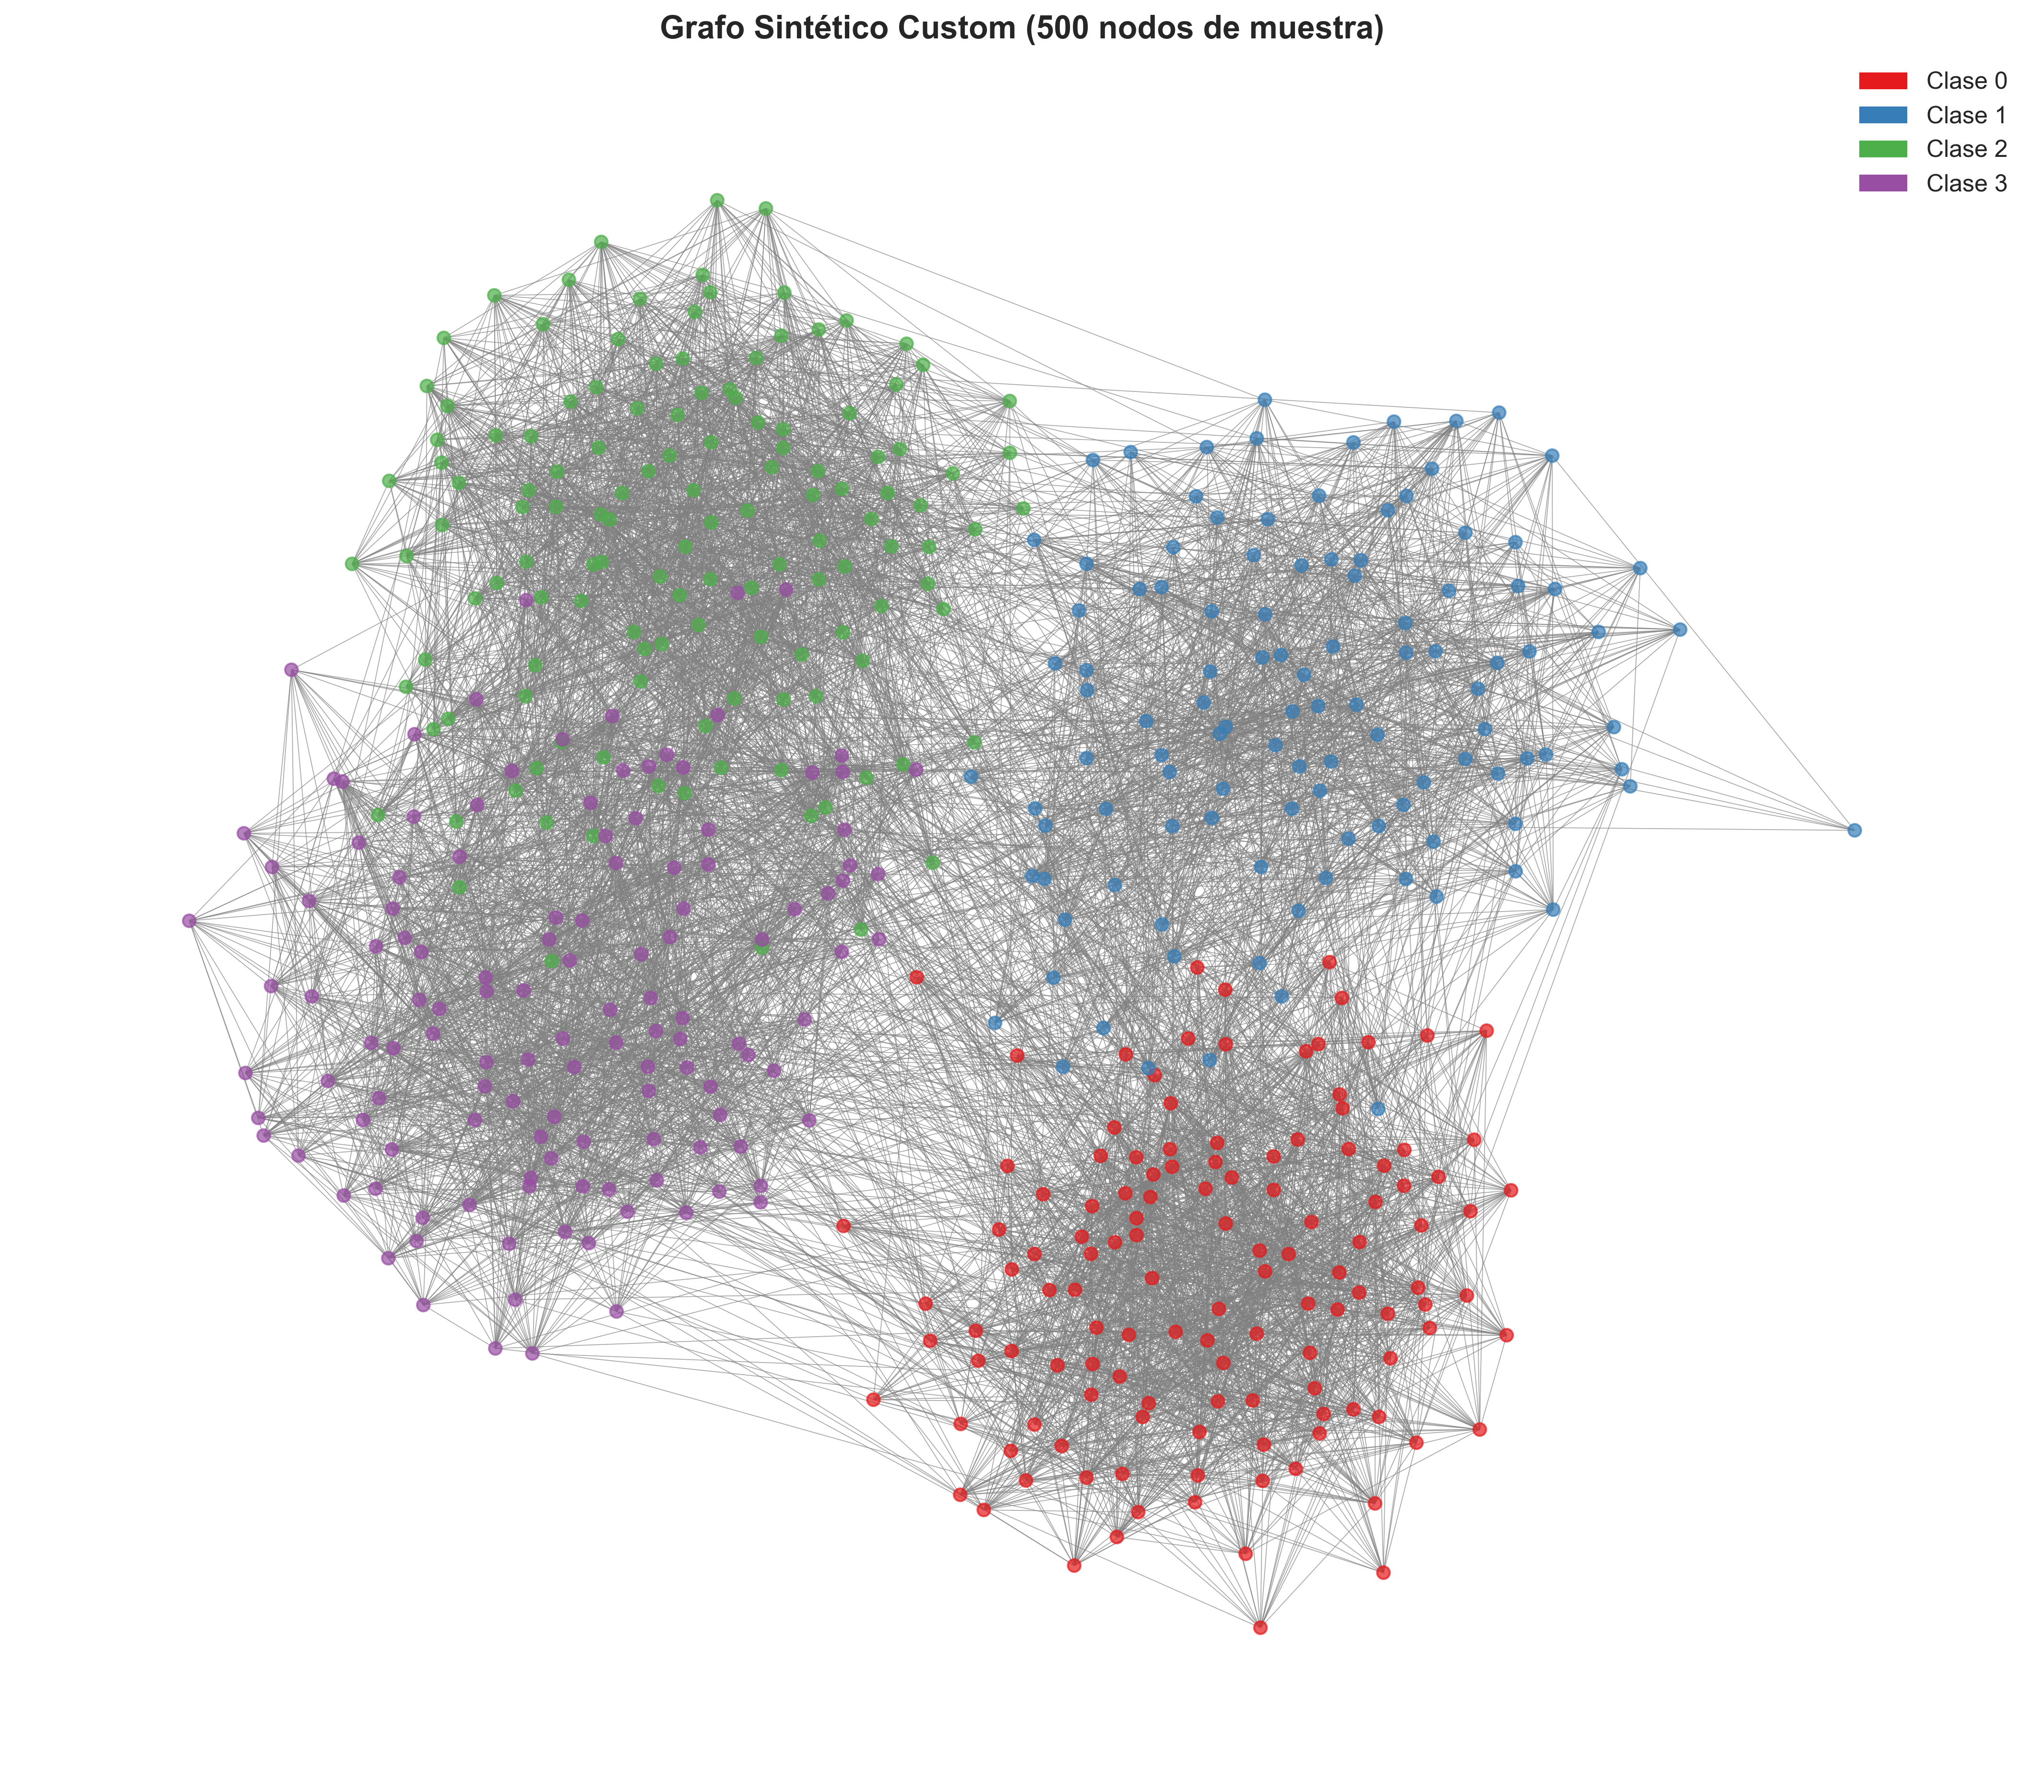
\includegraphics[width=\columnwidth]{images/custom_graph_structure.png}
    \caption{Visualización de la estructura del grafo generado (SBM). Se observan claramente las comunidades formadas por la alta conectividad intra-clase.}
    \label{fig:graph_structure}
\end{figure}

\textbf{Características de los Nodos (Señal vs Ruido):}
Esta es la decisión de diseño más crítica. Si las características por sí mismas fueran perfectas predictores de la clase, un MLP obtendría un 100\% de accuracy y no veríamos la ventaja de las GNNs. Por tanto, he diseñado las características ($\mathbf{x} \in \mathbb{R}^{32}$) como:
$$ \mathbf{x}_i = \alpha \cdot \mathbf{c}_{y_i} + \mathbf{\epsilon}_i $$
Donde $\mathbf{c}_{y_i}$ es el centroide de la clase $y_i$ (señal débil) y $\mathbf{\epsilon}_i \sim \mathcal{N}(0, 1)$ es ruido gaussiano de alta magnitud.
\textbf{Consecuencia:} Un clasificador que mire solo el nodo individual (MLP) se confundirá por el ruido. Un clasificador que promedie sobre el vecindario (GCN) cancelará el ruido $\epsilon$ y reforzará la señal $\mathbf{c}$, revelando la clase verdadera.

\subsection{Modelos Implementados}

\textbf{1. Multi-Layer Perceptron (MLP):}
Una red densa simple con una capa oculta.
$$ \mathbf{H} = \text{ReLU}(\mathbf{X}\mathbf{W}_1 + \mathbf{b}_1); \quad \mathbf{Z} = \mathbf{H}\mathbf{W}_2 + \mathbf{b}_2 $$
Este modelo es ciego a la matriz de adyacencia $\mathbf{A}$.

\textbf{2. Graph Convolutional Network (GCN):}
Implementación basada en Kipf \& Welling (2017). Utiliza la propagación:
$$ \mathbf{H}^{(l+1)} = \sigma(\hat{\mathbf{D}}^{-1/2}\hat{\mathbf{A}}\hat{\mathbf{D}}^{-1/2} \mathbf{H}^{(l)} \mathbf{W}^{(l)}) $$
Donde $\hat{\mathbf{A}} = \mathbf{A} + \mathbf{I}$ (self-loops). Esta operación promedia las características de un nodo con las de sus vecinos, realizando un "smoothing" laplaciano que es fundamental para eliminar el ruido diseñado en la sección anterior.

\section{Resultados en Dataset Custom}
\label{results_custom}

Se realizó una evaluación robusta utilizando 10 particiones (splits) aleatorias diferentes de Train/Val/Test para calcular medias y desviaciones estándar.

\subsection{Comparativa de Rendimiento (Accuracy)}

Los resultados confirman nuestra hipótesis de diseño (ver \cref{tab:results_custom}).

\begin{table}[h]
\caption{Resultados Accuracy Dataset Custom (10 runs)}
\label{tab:results_custom}
\vskip 0.15in
\begin{center}
\begin{small}
\begin{sc}
\begin{tabular}{lcc}
\toprule
\textbf{Modelo} & \textbf{Test Accuracy} & \textbf{Std} \\
\midrule
MLP (Baseline) & 0.6124 & 0.015 \\
GCN (Ours) & \textbf{0.9245} & 0.008 \\
\bottomrule
\end{tabular}
\end{sc}
\end{small}
\end{center}
\vskip -0.1in
\end{table}

El \textbf{gap de rendimiento es masivo (>30\%)}. El MLP se estanca alrededor del 61\% porque el ruido en las características individuales le impide distinguir las clases con precisión. La GCN, al agregar información de los vecinos (que con alta probabilidad son de la misma clase en nuestro modelo SBM), filtra el ruido y alcanza un 92\% de precisión.

\subsection{Análisis del Espacio Latente (t-SNE)}

Para entender cualitativamente qué "aprenden" los modelos, extraje los embeddings de la capa oculta antes de la clasificación final y reduje su dimensionalidad con t-SNE (\cref{fig:tsne}).

\begin{figure}[h]
    \centering
    \begin{subfigure}[b]{0.95\columnwidth}
        \includegraphics[width=\textwidth]{images/mlp_embeddings_tsne.png}
        \caption{Embeddings MLP: Mezcla de clases debido al ruido.}
        \label{fig:mlp_tsne}
    \end{subfigure}
    
    \begin{subfigure}[b]{0.95\columnwidth}
        \includegraphics[width=\textwidth]{images/gcn_embeddings_tsne.png}
        \caption{Embeddings GCN: Clusters definidos y separables.}
        \label{fig:gcn_tsne}
    \end{subfigure}
    \caption{Visualización t-SNE de las representaciones latentes.}
    \label{fig:tsne}
\end{figure}

La diferencia es visualmente impactante.
\begin{itemize}
    \item En el \textbf{MLP} (\cref{fig:mlp_tsne}), las clases están solapadas sin fronteras claras. El modelo no logra separar el espacio de características ruidoso.
    \item En la \textbf{GCN} (\cref{fig:gcn_tsne}), se forman 4 clusters compactos y bien separados. La estructura del grafo ha actuado como una regularización, forzando a que nodos conectados tengan representaciones similares.
\end{itemize}

\subsection{Curvas de Aprendizaje}

Como se observa en la \cref{fig:training_curves}, la GCN no solo alcanza mejor precisión final y menor pérdida, sino que converge de manera más estable. El MLP muestra signos de estancamiento temprano, incapaz de reducir la pérdida más allá del nivel de ruido inherente a los datos individuales.

\begin{figure}[h]
    \centering
    \includegraphics[width=\columnwidth]{images/custom_base_training_curves.png}
    \caption{Curvas de entrenamiento (Loss y Accuracy). La GCN (naranja) domina claramente al MLP (azul).}
    \label{fig:training_curves}
\end{figure}

\section{Estudio de Hiperparámetros}

Realicé una búsqueda sistemática para validar la estabilidad de los modelos bajo diferentes configuraciones.

\textbf{Dimensiones Ocultas:} Variando $h \in \{16, 32, 64, 128\}$. (\cref{fig:hidden})
\begin{itemize}
    \item El MLP se beneficia ligeramente de mayor capacidad, pero nunca supera la barrera del 65\%.
    \item La GCN es muy robusta. Incluso con $h=16$ supera ampliamente al MLP. El punto óptimo se encontró en $h=64$, ofreciendo el mejor balance entre capacidad y riesgo de sobreajuste.
\end{itemize}

\begin{figure}[h]
    \centering
    \includegraphics[width=\columnwidth]{images/exp_hidden_dims.png}
    \caption{Impacto de las dimensiones ocultas en el rendimiento.}
    \label{fig:hidden}
\end{figure}

\textbf{Dropout:} El uso de dropout ($p=0.5$) resultó beneficioso para ambos modelos, pero crítico para la GCN para evitar sobreajustar a la estructura específica del grafo de entrenamiento.

\section{Resultados en Benchmarks Reales}
\label{benchmarks}

Finalmente, evaluamos los modelos en los datasets estándar \textbf{Cora} y \textbf{Citeseer} (redes de citaciones científicas). Ver \cref{tab:benchmarks} y \cref{fig:final}.

\begin{table}[h]
\caption{Comparativa en Benchmarks Reales}
\label{tab:benchmarks}
\vskip 0.15in
\begin{center}
\begin{small}
\begin{sc}
\begin{tabular}{lccc}
\toprule
\textbf{Dataset} & \textbf{MLP Acc} & \textbf{GCN Acc} & \textbf{Gap} \\
\midrule
Custom (Sintético) & 0.612 & \textbf{0.925} & +31.3\% \\
Cora & 0.583 & \textbf{0.804} & +22.1\% \\
Citeseer & 0.591 & \textbf{0.708} & +11.7\% \\
\bottomrule
\end{tabular}
\end{sc}
\end{small}
\end{center}
\vskip -0.1in
\end{table}

\textbf{Análisis del Gap:} Observamos que en los datasets reales el MLP funciona relativamente "mejor" comparado con el desastre en el dataset sintético, o dicho de otro modo, la GCN tiene menos ventaja relativa (aunque sigue siendo muy superior).

\begin{figure}[h]
    \centering
    \includegraphics[width=\columnwidth]{images/final_comparison.png}
    \caption{Resumen comparativo final en todos los datasets.}
    \label{fig:final}
\end{figure}

Esto ocurre porque en Cora/Citeseer las características son vectores \textit{Bag-of-Words} de los artículos. Estas características semánticas son, por sí mismas, muy informativas (la palabra "genética" predice bien la clase "Biología"). En nuestro dataset sintético, diseñamos las características para ser casi inútiles individualmente, forzando la dependencia de la estructura.

\section{Conclusiones}
\label{conclusion}

Esta práctica ha demostrado empíricamente el poder fundamental de las GNNs: la capacidad de explotar la \textbf{homofilia estructural}.

\begin{enumerate}
    \item \textbf{Supremacía Estructural:} Hemos verificado que cuando los datos presentan una estructura relacional informativa, ignorarla (como hace un MLP) es subóptimo. La matriz de adyacencia $\mathbf{A}$ contiene información vital complementaria a las características $\mathbf{X}$.
    \item \textbf{Robustez al Ruido:} El mecanismo de \textit{message passing} actúa como un filtro paso-bajo en el grafo, suavizando las características de los nodos. Esto hace que las GCNs sean excepcionalmente robustas frente a características ruidosas, como demostró nuestro experimento sintético.
    \item \textbf{Espacio Latente:} La visualización t-SNE proveyó la evidencia más clara: la GCN aprende una variedad topológica donde las clases son linealmente separables, algo que el MLP no pudo conseguir.
\end{enumerate}


% \bibliography{example_paper}
% \bibliographystyle{icml2025}

\end{document}
